\documentclass[1p]{elsarticle_modified}
%\bibliographystyle{elsarticle-num}

%\usepackage[colorlinks]{hyperref}
%\usepackage{abbrmath_seonhwa} %\Abb, \Ascr, \Acal ,\Abf, \Afrak
\usepackage{amsfonts}
\usepackage{amssymb}
\usepackage{amsmath}
\usepackage{amsthm}
\usepackage{scalefnt}
\usepackage{amsbsy}
\usepackage{kotex}
\usepackage{caption}
\usepackage{subfig}
\usepackage{color}
\usepackage{graphicx}
\usepackage{xcolor} %% white, black, red, green, blue, cyan, magenta, yellow
\usepackage{float}
\usepackage{setspace}
\usepackage{hyperref}

\usepackage{tikz}
\usetikzlibrary{arrows}

\usepackage{multirow}
\usepackage{array} % fixed length table
\usepackage{hhline}

%%%%%%%%%%%%%%%%%%%%%
\makeatletter
\renewcommand*\env@matrix[1][\arraystretch]{%
	\edef\arraystretch{#1}%
	\hskip -\arraycolsep
	\let\@ifnextchar\new@ifnextchar
	\array{*\c@MaxMatrixCols c}}
\makeatother %https://tex.stackexchange.com/questions/14071/how-can-i-increase-the-line-spacing-in-a-matrix
%%%%%%%%%%%%%%%

\usepackage[normalem]{ulem}

\newcommand{\msout}[1]{\ifmmode\text{\sout{\ensuremath{#1}}}\else\sout{#1}\fi}
%SOURCE: \msout is \stkout macro in https://tex.stackexchange.com/questions/20609/strikeout-in-math-mode

\newcommand{\cancel}[1]{
	\ifmmode
	{\color{red}\msout{#1}}
	\else
	{\color{red}\sout{#1}}
	\fi
}

\newcommand{\add}[1]{
	{\color{blue}\uwave{#1}}
}

\newcommand{\replace}[2]{
	\ifmmode
	{\color{red}\msout{#1}}{\color{blue}\uwave{#2}}
	\else
	{\color{red}\sout{#1}}{\color{blue}\uwave{#2}}
	\fi
}

\newcommand{\Sol}{\mathcal{S}} %segment
\newcommand{\D}{D} %diagram
\newcommand{\A}{\mathcal{A}} %arc


%%%%%%%%%%%%%%%%%%%%%%%%%%%%%5 test

\def\sl{\operatorname{\textup{SL}}(2,\Cbb)}
\def\psl{\operatorname{\textup{PSL}}(2,\Cbb)}
\def\quan{\mkern 1mu \triangleright \mkern 1mu}

\theoremstyle{definition}
\newtheorem{thm}{Theorem}[section]
\newtheorem{prop}[thm]{Proposition}
\newtheorem{lem}[thm]{Lemma}
\newtheorem{ques}[thm]{Question}
\newtheorem{cor}[thm]{Corollary}
\newtheorem{defn}[thm]{Definition}
\newtheorem{exam}[thm]{Example}
\newtheorem{rmk}[thm]{Remark}
\newtheorem{alg}[thm]{Algorithm}

\newcommand{\I}{\sqrt{-1}}
\begin{document}

%\begin{frontmatter}
%
%\title{Boundary parabolic representations of knots up to 8 crossings}
%
%%% Group authors per affiliation:
%\author{Yunhi Cho} 
%\address{Department of Mathematics, University of Seoul, Seoul, Korea}
%\ead{yhcho@uos.ac.kr}
%
%
%\author{Seonhwa Kim} %\fnref{s_kim}}
%\address{Center for Geometry and Physics, Institute for Basic Science, Pohang, 37673, Korea}
%\ead{ryeona17@ibs.re.kr}
%
%\author{Hyuk Kim}
%\address{Department of Mathematical Sciences, Seoul National University, Seoul 08826, Korea}
%\ead{hyukkim@snu.ac.kr}
%
%\author{Seokbeom Yoon}
%\address{Department of Mathematical Sciences, Seoul National University, Seoul, 08826,  Korea}
%\ead{sbyoon15@snu.ac.kr}
%
%\begin{abstract}
%We find all boundary parabolic representation of knots up to 8 crossings.
%
%\end{abstract}
%\begin{keyword}
%    \MSC[2010] 57M25 
%\end{keyword}
%
%\end{frontmatter}

%\linenumbers
%\tableofcontents
%
\newcommand\colored[1]{\textcolor{white}{\rule[-0.35ex]{0.8em}{1.4ex}}\kern-0.8em\color{red} #1}%
%\newcommand\colored[1]{\textcolor{white}{ #1}\kern-2.17ex	\textcolor{white}{ #1}\kern-1.81ex	\textcolor{white}{ #1}\kern-2.15ex\color{red}#1	}

{\Large $\underline{12n_{0629}~(K12n_{0629})}$}

\setlength{\tabcolsep}{10pt}
\renewcommand{\arraystretch}{1.6}
\vspace{1cm}\begin{tabular}{m{100pt}>{\centering\arraybackslash}m{274pt}}
\multirow{5}{120pt}{
	\centering
	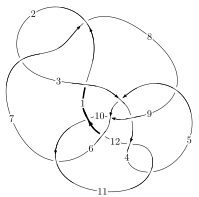
\includegraphics[width=112pt]{../../../GIT/diagram.site/Diagrams/png/2718_12n_0629.png}\\
\ \ \ A knot diagram\footnotemark}&
\allowdisplaybreaks
\textbf{Linearized knot diagam} \\
\cline{2-2}
 &
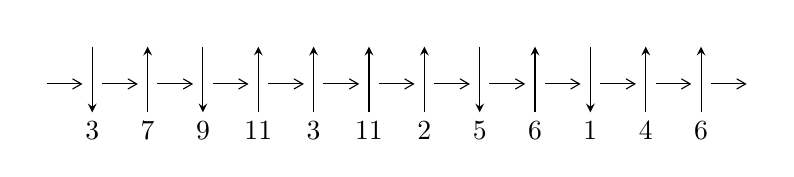
\begin{tikzpicture}[x=20pt, y=17pt]
	% nodes
	\node (C0) at (0, 0) {};
	\node (C1) at (1, 0) {};
	\node (C1U) at (1, +1) {};
	\node (C1D) at (1, -1) {3};

	\node (C2) at (2, 0) {};
	\node (C2U) at (2, +1) {};
	\node (C2D) at (2, -1) {7};

	\node (C3) at (3, 0) {};
	\node (C3U) at (3, +1) {};
	\node (C3D) at (3, -1) {9};

	\node (C4) at (4, 0) {};
	\node (C4U) at (4, +1) {};
	\node (C4D) at (4, -1) {11};

	\node (C5) at (5, 0) {};
	\node (C5U) at (5, +1) {};
	\node (C5D) at (5, -1) {3};

	\node (C6) at (6, 0) {};
	\node (C6U) at (6, +1) {};
	\node (C6D) at (6, -1) {11};

	\node (C7) at (7, 0) {};
	\node (C7U) at (7, +1) {};
	\node (C7D) at (7, -1) {2};

	\node (C8) at (8, 0) {};
	\node (C8U) at (8, +1) {};
	\node (C8D) at (8, -1) {5};

	\node (C9) at (9, 0) {};
	\node (C9U) at (9, +1) {};
	\node (C9D) at (9, -1) {6};

	\node (C10) at (10, 0) {};
	\node (C10U) at (10, +1) {};
	\node (C10D) at (10, -1) {1};

	\node (C11) at (11, 0) {};
	\node (C11U) at (11, +1) {};
	\node (C11D) at (11, -1) {4};

	\node (C12) at (12, 0) {};
	\node (C12U) at (12, +1) {};
	\node (C12D) at (12, -1) {6};
	\node (C13) at (13, 0) {};

	% arrows
	\draw[->,>={angle 60}]
	(C0) edge (C1) (C1) edge (C2) (C2) edge (C3) (C3) edge (C4) (C4) edge (C5) (C5) edge (C6) (C6) edge (C7) (C7) edge (C8) (C8) edge (C9) (C9) edge (C10) (C10) edge (C11) (C11) edge (C12) (C12) edge (C13) ;	\draw[->,>=stealth]
	(C1U) edge (C1D) (C2D) edge (C2U) (C3U) edge (C3D) (C4D) edge (C4U) (C5D) edge (C5U) (C6D) edge (C6U) (C7D) edge (C7U) (C8U) edge (C8D) (C9D) edge (C9U) (C10U) edge (C10D) (C11D) edge (C11U) (C12D) edge (C12U) ;
	\end{tikzpicture} \\
\hhline{~~} \\& 
\textbf{Solving Sequence} \\ \cline{2-2} 
 &
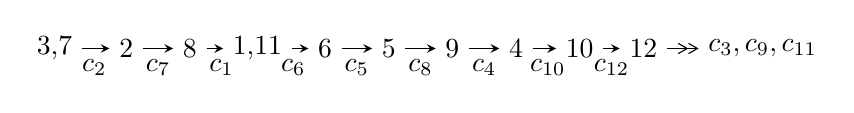
\begin{tikzpicture}[x=23pt, y=7pt]
	% node
	\node (A0) at (-1/8, 0) {3,7};
	\node (A1) at (1, 0) {2};
	\node (A2) at (2, 0) {8};
	\node (A3) at (49/16, 0) {1,11};
	\node (A4) at (33/8, 0) {6};
	\node (A5) at (41/8, 0) {5};
	\node (A6) at (49/8, 0) {9};
	\node (A7) at (57/8, 0) {4};
	\node (A8) at (65/8, 0) {10};
	\node (A9) at (73/8, 0) {12};
	\node (C1) at (1/2, -1) {$c_{2}$};
	\node (C2) at (3/2, -1) {$c_{7}$};
	\node (C3) at (5/2, -1) {$c_{1}$};
	\node (C4) at (29/8, -1) {$c_{6}$};
	\node (C5) at (37/8, -1) {$c_{5}$};
	\node (C6) at (45/8, -1) {$c_{8}$};
	\node (C7) at (53/8, -1) {$c_{4}$};
	\node (C8) at (61/8, -1) {$c_{10}$};
	\node (C9) at (69/8, -1) {$c_{12}$};
	\node (A10) at (11, 0) {$c_{3},c_{9},c_{11}$};

	% edge
	\draw[->,>=stealth]	
	(A0) edge (A1) (A1) edge (A2) (A2) edge (A3) (A3) edge (A4) (A4) edge (A5) (A5) edge (A6) (A6) edge (A7) (A7) edge (A8) (A8) edge (A9) ;
	\draw[->>,>={angle 60}]	
	(A9) edge (A10);
\end{tikzpicture} \\ 

\end{tabular} \\

\footnotetext{
The image of knot diagram is generated by the software ``\textbf{Draw programme}" developed by Andrew Bartholomew(\url{http://www.layer8.co.uk/maths/draw/index.htm\#Running-draw}), where we modified some parts for our purpose(\url{https://github.com/CATsTAILs/LinksPainter}).
}\phantom \\ \newline 
\centering \textbf{Ideals for irreducible components\footnotemark of $X_{\text{par}}$} 
 
\begin{align*}
I^u_{1}&=\langle 
979 u^{17}-284 u^{16}+\cdots+2700 b-1352,\;-3937 u^{17}-1528 u^{16}+\cdots+2700 a-754,\\
\phantom{I^u_{1}}&\phantom{= \langle  }u^{18}+8 u^{16}+\cdots- u+2\rangle \\
I^u_{2}&=\langle 
u^4- u^3+b- u-1,\;- u^4+a+u,\;u^5- u^4+u^3-2 u^2+u-1\rangle \\
I^u_{3}&=\langle 
44 u^{11}+41 u^{10}+\cdots+211 b+343,\;516 u^{11}+711 u^{10}+\cdots+1055 a+1970,\\
\phantom{I^u_{3}}&\phantom{= \langle  }u^{12}+u^{11}+8 u^{10}+8 u^9+26 u^8+23 u^7+44 u^6+30 u^5+41 u^4+18 u^3+19 u^2+5 u+5\rangle \\
I^u_{4}&=\langle 
-43712 u^{11}-79401 u^{10}+\cdots+207893 b-981135,\\
\phantom{I^u_{4}}&\phantom{= \langle  }-365996832 u^{11}-669919369 u^{10}+\cdots+1070441057 a-7841083848,\\
\phantom{I^u_{4}}&\phantom{= \langle  }u^{12}+u^{11}-4 u^{10}-2 u^9+16 u^8+3 u^7-26 u^6+4 u^5+5 u^4-10 u^3+3 u^2+29 u-19\rangle \\
\\
\end{align*}
\raggedright * 4 irreducible components of $\dim_{\mathbb{C}}=0$, with total 47 representations.\\
\footnotetext{All coefficients of polynomials are rational numbers. But the coefficients are sometimes approximated in decimal forms when there is not enough margin.}
\newpage
\renewcommand{\arraystretch}{1}
\centering \section*{I. $I^u_{1}= \langle 979 u^{17}-284 u^{16}+\cdots+2700 b-1352,\;-3937 u^{17}-1528 u^{16}+\cdots+2700 a-754,\;u^{18}+8 u^{16}+\cdots- u+2 \rangle$}
\flushleft \textbf{(i) Arc colorings}\\
\begin{tabular}{m{7pt} m{180pt} m{7pt} m{180pt} }
\flushright $a_{3}=$&$\begin{pmatrix}1\\0\end{pmatrix}$ \\
\flushright $a_{7}=$&$\begin{pmatrix}0\\u\end{pmatrix}$ \\
\flushright $a_{2}=$&$\begin{pmatrix}1\\u^2\end{pmatrix}$ \\
\flushright $a_{8}=$&$\begin{pmatrix}u\\u^3+u\end{pmatrix}$ \\
\flushright $a_{1}=$&$\begin{pmatrix}u^2+1\\u^2\end{pmatrix}$ \\
\flushright $a_{11}=$&$\begin{pmatrix}1.45815 u^{17}+0.565926 u^{16}+\cdots+9.00519 u+0.279259\\-0.362593 u^{17}+0.105185 u^{16}+\cdots-1.51407 u+0.500741\end{pmatrix}$ \\
\flushright $a_{6}=$&$\begin{pmatrix}0.813333 u^{17}+0.0700000 u^{16}+\cdots+3.31000 u-1.44000\\0.565926 u^{17}-0.386296 u^{16}+\cdots+1.73741 u-2.91630\end{pmatrix}$ \\
\flushright $a_{5}=$&$\begin{pmatrix}0.247407 u^{17}+0.456296 u^{16}+\cdots+1.57259 u+1.47630\\0.565926 u^{17}-0.386296 u^{16}+\cdots+1.73741 u-2.91630\end{pmatrix}$ \\
\flushright $a_{9}=$&$\begin{pmatrix}-0.312222 u^{17}+0.356667 u^{16}+\cdots-3.17444 u+1.40889\\0.396667 u^{17}+0.258889 u^{16}+\cdots+5.39333 u+0.604444\end{pmatrix}$ \\
\flushright $a_{4}=$&$\begin{pmatrix}-0.318519 u^{17}+0.842593 u^{16}+\cdots-0.164815 u+4.39259\\0.460741 u^{17}-0.529259 u^{16}+\cdots+1.59926 u-3.64148\end{pmatrix}$ \\
\flushright $a_{10}=$&$\begin{pmatrix}1.64704 u^{17}+0.910370 u^{16}+\cdots+10.6330 u+1.11259\\-0.340370 u^{17}+0.155185 u^{16}+\cdots-1.55296 u-0.0881481\end{pmatrix}$ \\
\flushright $a_{12}=$&$\begin{pmatrix}0.615556 u^{17}+0.228889 u^{16}+\cdots+4.93111 u-0.357778\\\frac{1}{6} u^{17}+\frac{53}{180} u^{16}+\cdots+\frac{5}{3} u+\frac{64}{45}\end{pmatrix}$\\&\end{tabular}
\flushleft \textbf{(ii) Obstruction class $= -1$}\\~\\
\flushleft \textbf{(iii) Cusp Shapes $= \frac{157}{27} u^{17}+\frac{70}{27} u^{16}+\cdots+\frac{1184}{27} u+\frac{34}{27}$}\\~\\
\newpage\renewcommand{\arraystretch}{1}
\flushleft \textbf{(iv) u-Polynomials at the component}\newline \\
\begin{tabular}{m{50pt}|m{274pt}}
Crossings & \hspace{64pt}u-Polynomials at each crossing \\
\hline $$\begin{aligned}c_{1}\end{aligned}$$&$\begin{aligned}
&u^{18}+16 u^{17}+\cdots+59 u+4
\end{aligned}$\\
\hline $$\begin{aligned}c_{2},c_{4},c_{7}\\c_{11}\end{aligned}$$&$\begin{aligned}
&u^{18}+8 u^{16}+\cdots+u+2
\end{aligned}$\\
\hline $$\begin{aligned}c_{3}\end{aligned}$$&$\begin{aligned}
&u^{18}-5 u^{17}+\cdots-27 u+9
\end{aligned}$\\
\hline $$\begin{aligned}c_{5},c_{6}\end{aligned}$$&$\begin{aligned}
&u^{18}+u^{17}+\cdots- u+1
\end{aligned}$\\
\hline $$\begin{aligned}c_{8}\end{aligned}$$&$\begin{aligned}
&u^{18}-3 u^{17}+\cdots-25 u+125
\end{aligned}$\\
\hline $$\begin{aligned}c_{9}\end{aligned}$$&$\begin{aligned}
&u^{18}-5 u^{17}+\cdots-125 u+46
\end{aligned}$\\
\hline $$\begin{aligned}c_{10}\end{aligned}$$&$\begin{aligned}
&u^{18}-2 u^{17}+\cdots+4 u+1
\end{aligned}$\\
\hline $$\begin{aligned}c_{12}\end{aligned}$$&$\begin{aligned}
&u^{18}+u^{17}+\cdots-160 u+32
\end{aligned}$\\
\hline
\end{tabular}\\~\\
\newpage\renewcommand{\arraystretch}{1}
\flushleft \textbf{(v) Riley Polynomials at the component}\newline \\
\begin{tabular}{m{50pt}|m{274pt}}
Crossings & \hspace{64pt}Riley Polynomials at each crossing \\
\hline $$\begin{aligned}c_{1}\end{aligned}$$&$\begin{aligned}
&y^{18}+12 y^{17}+\cdots+159 y+16
\end{aligned}$\\
\hline $$\begin{aligned}c_{2},c_{4},c_{7}\\c_{11}\end{aligned}$$&$\begin{aligned}
&y^{18}+16 y^{17}+\cdots+59 y+4
\end{aligned}$\\
\hline $$\begin{aligned}c_{3}\end{aligned}$$&$\begin{aligned}
&y^{18}-5 y^{17}+\cdots-117 y+81
\end{aligned}$\\
\hline $$\begin{aligned}c_{5},c_{6}\end{aligned}$$&$\begin{aligned}
&y^{18}-7 y^{17}+\cdots-11 y+1
\end{aligned}$\\
\hline $$\begin{aligned}c_{8}\end{aligned}$$&$\begin{aligned}
&y^{18}+11 y^{17}+\cdots+194375 y+15625
\end{aligned}$\\
\hline $$\begin{aligned}c_{9}\end{aligned}$$&$\begin{aligned}
&y^{18}+5 y^{17}+\cdots+21911 y+2116
\end{aligned}$\\
\hline $$\begin{aligned}c_{10}\end{aligned}$$&$\begin{aligned}
&y^{18}-8 y^{17}+\cdots+16 y+1
\end{aligned}$\\
\hline $$\begin{aligned}c_{12}\end{aligned}$$&$\begin{aligned}
&y^{18}+55 y^{17}+\cdots+10752 y+1024
\end{aligned}$\\
\hline
\end{tabular}\\~\\
\newpage\flushleft \textbf{(vi) Complex Volumes and Cusp Shapes}
$$\begin{array}{c|c|c}  
\text{Solutions to }I^u_{1}& \I (\text{vol} + \sqrt{-1}CS) & \text{Cusp shape}\\
 \hline 
\begin{aligned}
u &= -0.215825 + 1.055720 I \\
a &= -0.734208 - 0.778679 I \\
b &= -1.64100 + 0.67983 I\end{aligned}
 & -2.40740 - 4.93155 I & -0.09123 + 5.12585 I \\ \hline\begin{aligned}
u &= -0.215825 - 1.055720 I \\
a &= -0.734208 + 0.778679 I \\
b &= -1.64100 - 0.67983 I\end{aligned}
 & -2.40740 + 4.93155 I & -0.09123 - 5.12585 I \\ \hline\begin{aligned}
u &= \phantom{-}0.478183 + 1.019630 I \\
a &= \phantom{-}0.317066 - 0.189944 I \\
b &= \phantom{-}1.32096 + 1.39042 I\end{aligned}
 & -2.57674 + 6.69706 I & -4.74227 - 7.81204 I \\ \hline\begin{aligned}
u &= \phantom{-}0.478183 - 1.019630 I \\
a &= \phantom{-}0.317066 + 0.189944 I \\
b &= \phantom{-}1.32096 - 1.39042 I\end{aligned}
 & -2.57674 - 6.69706 I & -4.74227 + 7.81204 I \\ \hline\begin{aligned}
u &= -0.190193 + 1.174750 I \\
a &= \phantom{-}1.023770 - 0.233990 I \\
b &= -0.071711 + 0.212167 I\end{aligned}
 & -10.20590 - 2.87633 I & -5.03342 + 3.27746 I \\ \hline\begin{aligned}
u &= -0.190193 - 1.174750 I \\
a &= \phantom{-}1.023770 + 0.233990 I \\
b &= -0.071711 - 0.212167 I\end{aligned}
 & -10.20590 + 2.87633 I & -5.03342 - 3.27746 I \\ \hline\begin{aligned}
u &= \phantom{-}0.306395 + 0.502489 I \\
a &= -1.54759 - 1.06420 I \\
b &= -1.43872 + 0.30168 I\end{aligned}
 & -5.29960 + 1.10158 I & -0.68390 - 6.02655 I \\ \hline\begin{aligned}
u &= \phantom{-}0.306395 - 0.502489 I \\
a &= -1.54759 + 1.06420 I \\
b &= -1.43872 - 0.30168 I\end{aligned}
 & -5.29960 - 1.10158 I & -0.68390 + 6.02655 I \\ \hline\begin{aligned}
u &= -0.361458 + 0.449248 I \\
a &= \phantom{-}0.610707 + 0.324621 I \\
b &= \phantom{-}0.276717 - 0.678638 I\end{aligned}
 & \phantom{-}0.735931 - 0.874748 I & \phantom{-}7.31455 + 6.56056 I \\ \hline\begin{aligned}
u &= -0.361458 - 0.449248 I \\
a &= \phantom{-}0.610707 - 0.324621 I \\
b &= \phantom{-}0.276717 + 0.678638 I\end{aligned}
 & \phantom{-}0.735931 + 0.874748 I & \phantom{-}7.31455 - 6.56056 I\\
 \hline 
 \end{array}$$\newpage$$\begin{array}{c|c|c}  
\text{Solutions to }I^u_{1}& \I (\text{vol} + \sqrt{-1}CS) & \text{Cusp shape}\\
 \hline 
\begin{aligned}
u &= \phantom{-}0.106479 + 0.548573 I \\
a &= \phantom{-}0.36979 + 1.39973 I \\
b &= -0.823575 - 0.667813 I\end{aligned}
 & \phantom{-}0.97688 - 1.19294 I & \phantom{-}6.66369 + 7.49944 I \\ \hline\begin{aligned}
u &= \phantom{-}0.106479 - 0.548573 I \\
a &= \phantom{-}0.36979 - 1.39973 I \\
b &= -0.823575 + 0.667813 I\end{aligned}
 & \phantom{-}0.97688 + 1.19294 I & \phantom{-}6.66369 - 7.49944 I \\ \hline\begin{aligned}
u &= \phantom{-}1.06422 + 1.22609 I \\
a &= -1.204040 + 0.574237 I \\
b &= -1.67663 - 0.32270 I\end{aligned}
 & \phantom{-}8.00245 + 5.89453 I & \phantom{-}4.19834 - 2.56372 I \\ \hline\begin{aligned}
u &= \phantom{-}1.06422 - 1.22609 I \\
a &= -1.204040 - 0.574237 I \\
b &= -1.67663 + 0.32270 I\end{aligned}
 & \phantom{-}8.00245 - 5.89453 I & \phantom{-}4.19834 + 2.56372 I \\ \hline\begin{aligned}
u &= -0.07359 + 1.71354 I \\
a &= \phantom{-}0.542354 - 0.090003 I \\
b &= \phantom{-}0.794398 + 0.297779 I\end{aligned}
 & -13.22560 + 1.02068 I & -1.08623 - 7.18728 I \\ \hline\begin{aligned}
u &= -0.07359 - 1.71354 I \\
a &= \phantom{-}0.542354 + 0.090003 I \\
b &= \phantom{-}0.794398 - 0.297779 I\end{aligned}
 & -13.22560 - 1.02068 I & -1.08623 + 7.18728 I \\ \hline\begin{aligned}
u &= -1.11421 + 1.48248 I \\
a &= -1.127850 - 0.501165 I \\
b &= -1.74044 + 0.32902 I\end{aligned}
 & \phantom{-}6.7281 - 12.7161 I & \phantom{-}2.96048 + 6.03348 I \\ \hline\begin{aligned}
u &= -1.11421 - 1.48248 I \\
a &= -1.127850 + 0.501165 I \\
b &= -1.74044 - 0.32902 I\end{aligned}
 & \phantom{-}6.7281 + 12.7161 I & \phantom{-}2.96048 - 6.03348 I\\
 \hline 
 \end{array}$$\newpage\newpage\renewcommand{\arraystretch}{1}
\centering \section*{II. $I^u_{2}= \langle u^4- u^3+b- u-1,\;- u^4+a+u,\;u^5- u^4+u^3-2 u^2+u-1 \rangle$}
\flushleft \textbf{(i) Arc colorings}\\
\begin{tabular}{m{7pt} m{180pt} m{7pt} m{180pt} }
\flushright $a_{3}=$&$\begin{pmatrix}1\\0\end{pmatrix}$ \\
\flushright $a_{7}=$&$\begin{pmatrix}0\\u\end{pmatrix}$ \\
\flushright $a_{2}=$&$\begin{pmatrix}1\\u^2\end{pmatrix}$ \\
\flushright $a_{8}=$&$\begin{pmatrix}u\\u^3+u\end{pmatrix}$ \\
\flushright $a_{1}=$&$\begin{pmatrix}u^2+1\\u^2\end{pmatrix}$ \\
\flushright $a_{11}=$&$\begin{pmatrix}u^4- u\\- u^4+u^3+u+1\end{pmatrix}$ \\
\flushright $a_{6}=$&$\begin{pmatrix}- u^4- u^2+u\\- u^4+u^3- u^2+u-1\end{pmatrix}$ \\
\flushright $a_{5}=$&$\begin{pmatrix}- u^3+1\\- u^4+u^3- u^2+u-1\end{pmatrix}$ \\
\flushright $a_{9}=$&$\begin{pmatrix}u^4- u^3- u\\- u^4+u^3- u^2+2 u\end{pmatrix}$ \\
\flushright $a_{4}=$&$\begin{pmatrix}u^4-2 u^3+u^2- u+2\\- u^4+2 u^3-2 u^2+3 u-2\end{pmatrix}$ \\
\flushright $a_{10}=$&$\begin{pmatrix}2 u^4+u^2- u\\u^3+u+1\end{pmatrix}$ \\
\flushright $a_{12}=$&$\begin{pmatrix}u^2+1\\u^2\end{pmatrix}$\\&\end{tabular}
\flushleft \textbf{(ii) Obstruction class $= 1$}\\~\\
\flushleft \textbf{(iii) Cusp Shapes $= 4 u^4+2 u^3-5 u^2$}\\~\\
\newpage\renewcommand{\arraystretch}{1}
\flushleft \textbf{(iv) u-Polynomials at the component}\newline \\
\begin{tabular}{m{50pt}|m{274pt}}
Crossings & \hspace{64pt}u-Polynomials at each crossing \\
\hline $$\begin{aligned}c_{1},c_{10}\end{aligned}$$&$\begin{aligned}
&u^5- u^4- u^3+4 u^2-3 u+1
\end{aligned}$\\
\hline $$\begin{aligned}c_{2},c_{4}\end{aligned}$$&$\begin{aligned}
&u^5- u^4+u^3-2 u^2+u-1
\end{aligned}$\\
\hline $$\begin{aligned}c_{3}\end{aligned}$$&$\begin{aligned}
&u^5-4 u^4+8 u^3-9 u^2+6 u-1
\end{aligned}$\\
\hline $$\begin{aligned}c_{5},c_{9}\end{aligned}$$&$\begin{aligned}
&u^5-2 u^4- u^3+2 u^2-1
\end{aligned}$\\
\hline $$\begin{aligned}c_{6}\end{aligned}$$&$\begin{aligned}
&u^5+2 u^4- u^3-2 u^2+1
\end{aligned}$\\
\hline $$\begin{aligned}c_{7},c_{11}\end{aligned}$$&$\begin{aligned}
&u^5+u^4+u^3+2 u^2+u+1
\end{aligned}$\\
\hline $$\begin{aligned}c_{8}\end{aligned}$$&$\begin{aligned}
&u^5-2 u^4+2 u^3-3 u^2+2 u-1
\end{aligned}$\\
\hline $$\begin{aligned}c_{12}\end{aligned}$$&$\begin{aligned}
&u^5
\end{aligned}$\\
\hline
\end{tabular}\\~\\
\newpage\renewcommand{\arraystretch}{1}
\flushleft \textbf{(v) Riley Polynomials at the component}\newline \\
\begin{tabular}{m{50pt}|m{274pt}}
Crossings & \hspace{64pt}Riley Polynomials at each crossing \\
\hline $$\begin{aligned}c_{1},c_{10}\end{aligned}$$&$\begin{aligned}
&y^5-3 y^4+3 y^3-8 y^2+y-1
\end{aligned}$\\
\hline $$\begin{aligned}c_{2},c_{4},c_{7}\\c_{11}\end{aligned}$$&$\begin{aligned}
&y^5+y^4- y^3-4 y^2-3 y-1
\end{aligned}$\\
\hline $$\begin{aligned}c_{3}\end{aligned}$$&$\begin{aligned}
&y^5+4 y^3+7 y^2+18 y-1
\end{aligned}$\\
\hline $$\begin{aligned}c_{5},c_{6},c_{9}\end{aligned}$$&$\begin{aligned}
&y^5-6 y^4+9 y^3-8 y^2+4 y-1
\end{aligned}$\\
\hline $$\begin{aligned}c_{8}\end{aligned}$$&$\begin{aligned}
&y^5-4 y^3-5 y^2-2 y-1
\end{aligned}$\\
\hline $$\begin{aligned}c_{12}\end{aligned}$$&$\begin{aligned}
&y^5
\end{aligned}$\\
\hline
\end{tabular}\\~\\
\newpage\flushleft \textbf{(vi) Complex Volumes and Cusp Shapes}
$$\begin{array}{c|c|c}  
\text{Solutions to }I^u_{2}& \I (\text{vol} + \sqrt{-1}CS) & \text{Cusp shape}\\
 \hline 
\begin{aligned}
u &= -0.428550 + 1.039280 I \\
a &= \phantom{-}0.438694 + 0.557752 I \\
b &= \phantom{-}1.87122 - 1.10766 I\end{aligned}
 & -1.91329 - 6.77491 I & \phantom{-}7.14260 + 9.74210 I \\ \hline\begin{aligned}
u &= -0.428550 - 1.039280 I \\
a &= \phantom{-}0.438694 - 0.557752 I \\
b &= \phantom{-}1.87122 + 1.10766 I\end{aligned}
 & -1.91329 + 6.77491 I & \phantom{-}7.14260 - 9.74210 I \\ \hline\begin{aligned}
u &= \phantom{-}0.276511 + 0.728237 I \\
a &= -0.232705 - 1.093810 I \\
b &= \phantom{-}0.813922 + 0.874646 I\end{aligned}
 & \phantom{-}0.789751 - 0.607163 I & \phantom{-}1.60701 - 3.91429 I \\ \hline\begin{aligned}
u &= \phantom{-}0.276511 - 0.728237 I \\
a &= -0.232705 + 1.093810 I \\
b &= \phantom{-}0.813922 - 0.874646 I\end{aligned}
 & \phantom{-}0.789751 + 0.607163 I & \phantom{-}1.60701 + 3.91429 I \\ \hline\begin{aligned}
u &= \phantom{-}1.30408\phantom{ +0.000000I} \\
a &= \phantom{-}1.58802\phantom{ +0.000000I} \\
b &= \phantom{-}1.62971\phantom{ +0.000000I}\end{aligned}
 & \phantom{-}5.53695\phantom{ +0.000000I} & \phantom{-}7.50080\phantom{ +0.000000I}\\
 \hline 
 \end{array}$$\newpage\newpage\renewcommand{\arraystretch}{1}
\centering \section*{III. $I^u_{3}= \langle 44 u^{11}+41 u^{10}+\cdots+211 b+343,\;516 u^{11}+711 u^{10}+\cdots+1055 a+1970,\;u^{12}+u^{11}+\cdots+5 u+5 \rangle$}
\flushleft \textbf{(i) Arc colorings}\\
\begin{tabular}{m{7pt} m{180pt} m{7pt} m{180pt} }
\flushright $a_{3}=$&$\begin{pmatrix}1\\0\end{pmatrix}$ \\
\flushright $a_{7}=$&$\begin{pmatrix}0\\u\end{pmatrix}$ \\
\flushright $a_{2}=$&$\begin{pmatrix}1\\u^2\end{pmatrix}$ \\
\flushright $a_{8}=$&$\begin{pmatrix}u\\u^3+u\end{pmatrix}$ \\
\flushright $a_{1}=$&$\begin{pmatrix}u^2+1\\u^2\end{pmatrix}$ \\
\flushright $a_{11}=$&$\begin{pmatrix}-0.489100 u^{11}-0.673934 u^{10}+\cdots-2.94692 u-1.86730\\-0.208531 u^{11}-0.194313 u^{10}+\cdots-2.45024 u-1.62559\end{pmatrix}$ \\
\flushright $a_{6}=$&$\begin{pmatrix}-0.0796209 u^{11}+0.0530806 u^{10}+\cdots-7.73555 u-1.83886\\-0.00473934 u^{11}+0.336493 u^{10}+\cdots-1.80569 u+0.985782\end{pmatrix}$ \\
\flushright $a_{5}=$&$\begin{pmatrix}-0.0748815 u^{11}-0.283412 u^{10}+\cdots-5.92986 u-2.82464\\-0.00473934 u^{11}+0.336493 u^{10}+\cdots-1.80569 u+0.985782\end{pmatrix}$ \\
\flushright $a_{9}=$&$\begin{pmatrix}0.176303 u^{11}+0.882464 u^{10}+\cdots+9.77156 u+3.92891\\0.374408 u^{11}+0.417062 u^{10}+\cdots+3.64929 u+2.12322\end{pmatrix}$ \\
\flushright $a_{4}=$&$\begin{pmatrix}0.249289 u^{11}-0.499526 u^{10}+\cdots-9.22085 u-6.05213\\0.199052 u^{11}-0.132701 u^{10}+\cdots-1.16114 u-1.40284\end{pmatrix}$ \\
\flushright $a_{10}=$&$\begin{pmatrix}-0.863507 u^{11}-1.09100 u^{10}+\cdots-4.59621 u-3.99052\\-0.0426540 u^{11}+0.0284360 u^{10}+\cdots+0.748815 u-1.12796\end{pmatrix}$ \\
\flushright $a_{12}=$&$\begin{pmatrix}0.367773 u^{11}+1.08815 u^{10}+\cdots+5.92133 u-1.69668\\-0.341232 u^{11}+0.227488 u^{10}+\cdots-1.00948 u-1.02370\end{pmatrix}$\\&\end{tabular}
\flushleft \textbf{(ii) Obstruction class $= 1$}\\~\\
\flushleft \textbf{(iii) Cusp Shapes $= -\frac{316}{211} u^{11}-\frac{352}{211} u^{10}-\frac{2504}{211} u^9-\frac{2856}{211} u^8-\frac{7676}{211} u^7-\frac{8260}{211} u^6-\frac{11672}{211} u^5-\frac{10564}{211} u^4-\frac{9416}{211} u^3-\frac{6312}{211} u^2-\frac{3080}{211} u-\frac{1581}{211}$}\\~\\
\newpage\renewcommand{\arraystretch}{1}
\flushleft \textbf{(iv) u-Polynomials at the component}\newline \\
\begin{tabular}{m{50pt}|m{274pt}}
Crossings & \hspace{64pt}u-Polynomials at each crossing \\
\hline $$\begin{aligned}c_{1}\end{aligned}$$&$\begin{aligned}
&u^{12}-15 u^{11}+\cdots-165 u+25
\end{aligned}$\\
\hline $$\begin{aligned}c_{2},c_{4}\end{aligned}$$&$\begin{aligned}
&u^{12}+u^{11}+\cdots+5 u+5
\end{aligned}$\\
\hline $$\begin{aligned}c_{3}\end{aligned}$$&$\begin{aligned}
&(u^3+u^2-1)^4
\end{aligned}$\\
\hline $$\begin{aligned}c_{5}\end{aligned}$$&$\begin{aligned}
&u^{12}+u^{11}+\cdots+2 u+1
\end{aligned}$\\
\hline $$\begin{aligned}c_{6}\end{aligned}$$&$\begin{aligned}
&u^{12}- u^{11}+\cdots-2 u+1
\end{aligned}$\\
\hline $$\begin{aligned}c_{7},c_{11}\end{aligned}$$&$\begin{aligned}
&u^{12}- u^{11}+\cdots-5 u+5
\end{aligned}$\\
\hline $$\begin{aligned}c_{8}\end{aligned}$$&$\begin{aligned}
&u^{12}-3 u^{11}+\cdots-54 u+121
\end{aligned}$\\
\hline $$\begin{aligned}c_{9}\end{aligned}$$&$\begin{aligned}
&u^{12}- u^{11}+\cdots+965 u+475
\end{aligned}$\\
\hline $$\begin{aligned}c_{10}\end{aligned}$$&$\begin{aligned}
&u^{12}-3 u^{11}+\cdots+6 u+1
\end{aligned}$\\
\hline $$\begin{aligned}c_{12}\end{aligned}$$&$\begin{aligned}
&u^{12}+21 u^{10}+135 u^8+300 u^6-65 u^4-214 u^2+661
\end{aligned}$\\
\hline
\end{tabular}\\~\\
\newpage\renewcommand{\arraystretch}{1}
\flushleft \textbf{(v) Riley Polynomials at the component}\newline \\
\begin{tabular}{m{50pt}|m{274pt}}
Crossings & \hspace{64pt}Riley Polynomials at each crossing \\
\hline $$\begin{aligned}c_{1}\end{aligned}$$&$\begin{aligned}
&y^{12}-25 y^{11}+\cdots+2325 y+625
\end{aligned}$\\
\hline $$\begin{aligned}c_{2},c_{4},c_{7}\\c_{11}\end{aligned}$$&$\begin{aligned}
&y^{12}+15 y^{11}+\cdots+165 y+25
\end{aligned}$\\
\hline $$\begin{aligned}c_{3}\end{aligned}$$&$\begin{aligned}
&(y^3- y^2+2 y-1)^4
\end{aligned}$\\
\hline $$\begin{aligned}c_{5},c_{6}\end{aligned}$$&$\begin{aligned}
&y^{12}+9 y^{11}+\cdots+2 y+1
\end{aligned}$\\
\hline $$\begin{aligned}c_{8}\end{aligned}$$&$\begin{aligned}
&y^{12}-19 y^{11}+\cdots+15718 y+14641
\end{aligned}$\\
\hline $$\begin{aligned}c_{9}\end{aligned}$$&$\begin{aligned}
&y^{12}+5 y^{11}+\cdots+820575 y+225625
\end{aligned}$\\
\hline $$\begin{aligned}c_{10}\end{aligned}$$&$\begin{aligned}
&y^{12}-13 y^{11}+\cdots+24 y+1
\end{aligned}$\\
\hline $$\begin{aligned}c_{12}\end{aligned}$$&$\begin{aligned}
&(y^6+21 y^5+135 y^4+300 y^3-65 y^2-214 y+661)^2
\end{aligned}$\\
\hline
\end{tabular}\\~\\
\newpage\flushleft \textbf{(vi) Complex Volumes and Cusp Shapes}
$$\begin{array}{c|c|c}  
\text{Solutions to }I^u_{3}& \I (\text{vol} + \sqrt{-1}CS) & \text{Cusp shape}\\
 \hline 
\begin{aligned}
u &= -0.656577 + 0.856222 I \\
a &= -0.535394 - 0.579005 I \\
b &= -1.61803\phantom{ +0.000000I}\end{aligned}
 & -1.25270 + 2.82812 I & \phantom{-}4.50976 - 2.97945 I \\ \hline\begin{aligned}
u &= -0.656577 - 0.856222 I \\
a &= -0.535394 + 0.579005 I \\
b &= -1.61803\phantom{ +0.000000I}\end{aligned}
 & -1.25270 - 2.82812 I & \phantom{-}4.50976 + 2.97945 I \\ \hline\begin{aligned}
u &= -0.461010 + 0.702960 I \\
a &= -1.246290 + 0.566838 I \\
b &= -1.61803\phantom{ +0.000000I}\end{aligned}
 & -5.39028\phantom{ +0.000000I} & -2.01951 + 0. I\phantom{ +0.000000I} \\ \hline\begin{aligned}
u &= -0.461010 - 0.702960 I \\
a &= -1.246290 - 0.566838 I \\
b &= -1.61803\phantom{ +0.000000I}\end{aligned}
 & -5.39028\phantom{ +0.000000I} & -2.01951 + 0. I\phantom{ +0.000000I} \\ \hline\begin{aligned}
u &= \phantom{-}0.301588 + 0.677598 I \\
a &= \phantom{-}2.11023 + 0.98157 I \\
b &= \phantom{-}0.618034\phantom{ +0.000000I}\end{aligned}
 & -9.14838 + 2.82812 I & \phantom{-}4.50976 - 2.97945 I \\ \hline\begin{aligned}
u &= \phantom{-}0.301588 - 0.677598 I \\
a &= \phantom{-}2.11023 - 0.98157 I \\
b &= \phantom{-}0.618034\phantom{ +0.000000I}\end{aligned}
 & -9.14838 - 2.82812 I & \phantom{-}4.50976 + 2.97945 I \\ \hline\begin{aligned}
u &= \phantom{-}0.308571 + 1.258780 I \\
a &= -0.677986 + 0.401303 I \\
b &= -1.61803\phantom{ +0.000000I}\end{aligned}
 & -1.25270 + 2.82812 I & \phantom{-}4.50976 - 2.97945 I \\ \hline\begin{aligned}
u &= \phantom{-}0.308571 - 1.258780 I \\
a &= -0.677986 - 0.401303 I \\
b &= -1.61803\phantom{ +0.000000I}\end{aligned}
 & -1.25270 - 2.82812 I & \phantom{-}4.50976 + 2.97945 I \\ \hline\begin{aligned}
u &= -0.16866 + 1.48546 I \\
a &= -0.234496 + 0.241588 I \\
b &= \phantom{-}0.618034\phantom{ +0.000000I}\end{aligned}
 & -9.14838 - 2.82812 I & \phantom{-}4.50976 + 2.97945 I \\ \hline\begin{aligned}
u &= -0.16866 - 1.48546 I \\
a &= -0.234496 - 0.241588 I \\
b &= \phantom{-}0.618034\phantom{ +0.000000I}\end{aligned}
 & -9.14838 + 2.82812 I & \phantom{-}4.50976 - 2.97945 I\\
 \hline 
 \end{array}$$\newpage$$\begin{array}{c|c|c}  
\text{Solutions to }I^u_{3}& \I (\text{vol} + \sqrt{-1}CS) & \text{Cusp shape}\\
 \hline 
\begin{aligned}
u &= \phantom{-}0.17609 + 1.70638 I \\
a &= \phantom{-}0.583936 + 0.330427 I \\
b &= \phantom{-}0.618034\phantom{ +0.000000I}\end{aligned}
 & -13.2860\phantom{ +0.000000I} & -2.01951 + 0. I\phantom{ +0.000000I} \\ \hline\begin{aligned}
u &= \phantom{-}0.17609 - 1.70638 I \\
a &= \phantom{-}0.583936 - 0.330427 I \\
b &= \phantom{-}0.618034\phantom{ +0.000000I}\end{aligned}
 & -13.2860\phantom{ +0.000000I} & -2.01951 + 0. I\phantom{ +0.000000I}\\
 \hline 
 \end{array}$$\newpage\newpage\renewcommand{\arraystretch}{1}
\centering \section*{IV. $I^u_{4}= \langle -4.37\times10^{4} u^{11}-7.94\times10^{4} u^{10}+\cdots+2.08\times10^{5} b-9.81\times10^{5},\;-3.66\times10^{8} u^{11}-6.70\times10^{8} u^{10}+\cdots+1.07\times10^{9} a-7.84\times10^{9},\;u^{12}+u^{11}+\cdots+29 u-19 \rangle$}
\flushleft \textbf{(i) Arc colorings}\\
\begin{tabular}{m{7pt} m{180pt} m{7pt} m{180pt} }
\flushright $a_{3}=$&$\begin{pmatrix}1\\0\end{pmatrix}$ \\
\flushright $a_{7}=$&$\begin{pmatrix}0\\u\end{pmatrix}$ \\
\flushright $a_{2}=$&$\begin{pmatrix}1\\u^2\end{pmatrix}$ \\
\flushright $a_{8}=$&$\begin{pmatrix}u\\u^3+u\end{pmatrix}$ \\
\flushright $a_{1}=$&$\begin{pmatrix}u^2+1\\u^2\end{pmatrix}$ \\
\flushright $a_{11}=$&$\begin{pmatrix}0.341912 u^{11}+0.625835 u^{10}+\cdots-2.65709 u+7.32510\\0.210262 u^{11}+0.381932 u^{10}+\cdots-1.21740 u+4.71942\end{pmatrix}$ \\
\flushright $a_{6}=$&$\begin{pmatrix}-0.467649 u^{11}-0.798651 u^{10}+\cdots+2.93801 u-11.4944\\-0.219258 u^{11}-0.339998 u^{10}+\cdots+1.34725 u-5.50844\end{pmatrix}$ \\
\flushright $a_{5}=$&$\begin{pmatrix}-0.248391 u^{11}-0.458653 u^{10}+\cdots+1.59076 u-5.98593\\-0.219258 u^{11}-0.339998 u^{10}+\cdots+1.34725 u-5.50844\end{pmatrix}$ \\
\flushright $a_{9}=$&$\begin{pmatrix}-0.141181 u^{11}-0.201538 u^{10}+\cdots+1.25160 u-3.49743\\-0.0951718 u^{11}-0.139896 u^{10}+\cdots+0.138622 u-2.31389\end{pmatrix}$ \\
\flushright $a_{4}=$&$\begin{pmatrix}0.164884 u^{11}+0.311952 u^{10}+\cdots-1.05429 u+4.02767\\0.112253 u^{11}+0.259321 u^{10}+\cdots-1.21218 u+2.50135\end{pmatrix}$ \\
\flushright $a_{10}=$&$\begin{pmatrix}0.353204 u^{11}+0.612703 u^{10}+\cdots-3.01116 u+10.6267\\0.158360 u^{11}+0.267974 u^{10}+\cdots-1.10804 u+5.43443\end{pmatrix}$ \\
\flushright $a_{12}=$&$\begin{pmatrix}0.511091 u^{11}+0.907271 u^{10}+\cdots-2.97620 u+12.2196\\0.299785 u^{11}+0.536124 u^{10}+\cdots-1.58475 u+6.27294\end{pmatrix}$\\&\end{tabular}
\flushleft \textbf{(ii) Obstruction class $= -1$}\\~\\
\flushleft \textbf{(iii) Cusp Shapes $= -\frac{1261620}{3314059} u^{11}-\frac{264928}{473437} u^{10}+\cdots+\frac{1837608}{3314059} u-\frac{27359429}{3314059}$}\\~\\
\newpage\renewcommand{\arraystretch}{1}
\flushleft \textbf{(iv) u-Polynomials at the component}\newline \\
\begin{tabular}{m{50pt}|m{274pt}}
Crossings & \hspace{64pt}u-Polynomials at each crossing \\
\hline $$\begin{aligned}c_{1}\end{aligned}$$&$\begin{aligned}
&u^{12}-9 u^{11}+\cdots-955 u+361
\end{aligned}$\\
\hline $$\begin{aligned}c_{2},c_{4},c_{7}\\c_{11}\end{aligned}$$&$\begin{aligned}
&u^{12}- u^{11}+\cdots-29 u-19
\end{aligned}$\\
\hline $$\begin{aligned}c_{3}\end{aligned}$$&$\begin{aligned}
&(u^3+u^2-1)^4
\end{aligned}$\\
\hline $$\begin{aligned}c_{5},c_{6}\end{aligned}$$&$\begin{aligned}
&u^{12}+u^{11}+\cdots-424 u-181
\end{aligned}$\\
\hline $$\begin{aligned}c_{8}\end{aligned}$$&$\begin{aligned}
&u^{12}+3 u^{11}+\cdots+1122 u+289
\end{aligned}$\\
\hline $$\begin{aligned}c_{9}\end{aligned}$$&$\begin{aligned}
&u^{12}+u^{11}+\cdots-33 u-19
\end{aligned}$\\
\hline $$\begin{aligned}c_{10}\end{aligned}$$&$\begin{aligned}
&u^{12}-3 u^{11}+\cdots+30 u+101
\end{aligned}$\\
\hline $$\begin{aligned}c_{12}\end{aligned}$$&$\begin{aligned}
&(u^6- u^5+5 u^4-2 u^3+u^2-2 u-1)^2
\end{aligned}$\\
\hline
\end{tabular}\\~\\
\newpage\renewcommand{\arraystretch}{1}
\flushleft \textbf{(v) Riley Polynomials at the component}\newline \\
\begin{tabular}{m{50pt}|m{274pt}}
Crossings & \hspace{64pt}Riley Polynomials at each crossing \\
\hline $$\begin{aligned}c_{1}\end{aligned}$$&$\begin{aligned}
&y^{12}+23 y^{11}+\cdots-623947 y+130321
\end{aligned}$\\
\hline $$\begin{aligned}c_{2},c_{4},c_{7}\\c_{11}\end{aligned}$$&$\begin{aligned}
&y^{12}-9 y^{11}+\cdots-955 y+361
\end{aligned}$\\
\hline $$\begin{aligned}c_{3}\end{aligned}$$&$\begin{aligned}
&(y^3- y^2+2 y-1)^4
\end{aligned}$\\
\hline $$\begin{aligned}c_{5},c_{6}\end{aligned}$$&$\begin{aligned}
&y^{12}-27 y^{11}+\cdots+27650 y+32761
\end{aligned}$\\
\hline $$\begin{aligned}c_{8}\end{aligned}$$&$\begin{aligned}
&y^{12}+25 y^{11}+\cdots-261834 y+83521
\end{aligned}$\\
\hline $$\begin{aligned}c_{9}\end{aligned}$$&$\begin{aligned}
&y^{12}-15 y^{11}+\cdots-481 y+361
\end{aligned}$\\
\hline $$\begin{aligned}c_{10}\end{aligned}$$&$\begin{aligned}
&y^{12}+11 y^{11}+\cdots+12836 y+10201
\end{aligned}$\\
\hline $$\begin{aligned}c_{12}\end{aligned}$$&$\begin{aligned}
&(y^6+9 y^5+23 y^4-17 y^2-6 y+1)^2
\end{aligned}$\\
\hline
\end{tabular}\\~\\
\newpage\flushleft \textbf{(vi) Complex Volumes and Cusp Shapes}
$$\begin{array}{c|c|c}  
\text{Solutions to }I^u_{4}& \I (\text{vol} + \sqrt{-1}CS) & \text{Cusp shape}\\
 \hline 
\begin{aligned}
u &= \phantom{-}0.176090 + 0.954853 I \\
a &= -0.511597 - 0.577155 I \\
b &= -0.618034\phantom{ +0.000000I}\end{aligned}
 & -3.41636\phantom{ +0.000000I} & -2.01951 + 0. I\phantom{ +0.000000I} \\ \hline\begin{aligned}
u &= \phantom{-}0.176090 - 0.954853 I \\
a &= -0.511597 + 0.577155 I \\
b &= -0.618034\phantom{ +0.000000I}\end{aligned}
 & -3.41636\phantom{ +0.000000I} & -2.01951 + 0. I\phantom{ +0.000000I} \\ \hline\begin{aligned}
u &= \phantom{-}1.042890 + 0.143496 I \\
a &= -0.246377 + 1.202250 I \\
b &= -0.618034\phantom{ +0.000000I}\end{aligned}
 & \phantom{-}0.72122 - 2.82812 I & \phantom{-}4.50976 + 2.97945 I \\ \hline\begin{aligned}
u &= \phantom{-}1.042890 - 0.143496 I \\
a &= -0.246377 - 1.202250 I \\
b &= -0.618034\phantom{ +0.000000I}\end{aligned}
 & \phantom{-}0.72122 + 2.82812 I & \phantom{-}4.50976 - 2.97945 I \\ \hline\begin{aligned}
u &= -0.909963 + 0.664361 I \\
a &= -0.088103 - 1.049580 I \\
b &= -0.618034\phantom{ +0.000000I}\end{aligned}
 & \phantom{-}0.72122 - 2.82812 I & \phantom{-}4.50976 + 2.97945 I \\ \hline\begin{aligned}
u &= -0.909963 - 0.664361 I \\
a &= -0.088103 + 1.049580 I \\
b &= -0.618034\phantom{ +0.000000I}\end{aligned}
 & \phantom{-}0.72122 + 2.82812 I & \phantom{-}4.50976 - 2.97945 I \\ \hline\begin{aligned}
u &= \phantom{-}0.766119\phantom{ +0.000000I} \\
a &= \phantom{-}2.36184\phantom{ +0.000000I} \\
b &= \phantom{-}1.61803\phantom{ +0.000000I}\end{aligned}
 & \phantom{-}4.47932\phantom{ +0.000000I} & -2.01950\phantom{ +0.000000I} \\ \hline\begin{aligned}
u &= -1.68814\phantom{ +0.000000I} \\
a &= \phantom{-}1.28048\phantom{ +0.000000I} \\
b &= \phantom{-}1.61803\phantom{ +0.000000I}\end{aligned}
 & \phantom{-}4.47932\phantom{ +0.000000I} & -2.01950\phantom{ +0.000000I} \\ \hline\begin{aligned}
u &= \phantom{-}1.30811 + 1.12304 I \\
a &= \phantom{-}1.218820 - 0.656524 I \\
b &= \phantom{-}1.61803\phantom{ +0.000000I}\end{aligned}
 & \phantom{-}8.61690 + 2.82812 I & \phantom{-}4.50976 - 2.97945 I \\ \hline\begin{aligned}
u &= \phantom{-}1.30811 - 1.12304 I \\
a &= \phantom{-}1.218820 + 0.656524 I \\
b &= \phantom{-}1.61803\phantom{ +0.000000I}\end{aligned}
 & \phantom{-}8.61690 - 2.82812 I & \phantom{-}4.50976 + 2.97945 I\\
 \hline 
 \end{array}$$\newpage$$\begin{array}{c|c|c}  
\text{Solutions to }I^u_{4}& \I (\text{vol} + \sqrt{-1}CS) & \text{Cusp shape}\\
 \hline 
\begin{aligned}
u &= -1.65612 + 0.99196 I \\
a &= \phantom{-}1.174520 + 0.523632 I \\
b &= \phantom{-}1.61803\phantom{ +0.000000I}\end{aligned}
 & \phantom{-}8.61690 + 2.82812 I & \phantom{-}4.50976 - 2.97945 I \\ \hline\begin{aligned}
u &= -1.65612 - 0.99196 I \\
a &= \phantom{-}1.174520 - 0.523632 I \\
b &= \phantom{-}1.61803\phantom{ +0.000000I}\end{aligned}
 & \phantom{-}8.61690 - 2.82812 I & \phantom{-}4.50976 + 2.97945 I\\
 \hline 
 \end{array}$$\newpage
\newpage\renewcommand{\arraystretch}{1}
\centering \section*{ V. u-Polynomials}
\begin{tabular}{m{50pt}|m{274pt}}
Crossings & \hspace{64pt}u-Polynomials at each crossing \\
\hline $$\begin{aligned}c_{1}\end{aligned}$$&$\begin{aligned}
&(u^5- u^4- u^3+4 u^2-3 u+1)(u^{12}-15 u^{11}+\cdots-165 u+25)\\
&\cdot(u^{12}-9 u^{11}+\cdots-955 u+361)(u^{18}+16 u^{17}+\cdots+59 u+4)
\end{aligned}$\\
\hline $$\begin{aligned}c_{2},c_{4}\end{aligned}$$&$\begin{aligned}
&(u^5- u^4+u^3-2 u^2+u-1)(u^{12}- u^{11}+\cdots-29 u-19)\\
&\cdot(u^{12}+u^{11}+\cdots+5 u+5)(u^{18}+8 u^{16}+\cdots+u+2)
\end{aligned}$\\
\hline $$\begin{aligned}c_{3}\end{aligned}$$&$\begin{aligned}
&(u^3+u^2-1)^8(u^5-4 u^4+8 u^3-9 u^2+6 u-1)\\
&\cdot(u^{18}-5 u^{17}+\cdots-27 u+9)
\end{aligned}$\\
\hline $$\begin{aligned}c_{5}\end{aligned}$$&$\begin{aligned}
&(u^5-2 u^4- u^3+2 u^2-1)(u^{12}+u^{11}+\cdots-424 u-181)\\
&\cdot(u^{12}+u^{11}+\cdots+2 u+1)(u^{18}+u^{17}+\cdots- u+1)
\end{aligned}$\\
\hline $$\begin{aligned}c_{6}\end{aligned}$$&$\begin{aligned}
&(u^5+2 u^4- u^3-2 u^2+1)(u^{12}- u^{11}+\cdots-2 u+1)\\
&\cdot(u^{12}+u^{11}+\cdots-424 u-181)(u^{18}+u^{17}+\cdots- u+1)
\end{aligned}$\\
\hline $$\begin{aligned}c_{7},c_{11}\end{aligned}$$&$\begin{aligned}
&(u^5+u^4+u^3+2 u^2+u+1)(u^{12}- u^{11}+\cdots-29 u-19)\\
&\cdot(u^{12}- u^{11}+\cdots-5 u+5)(u^{18}+8 u^{16}+\cdots+u+2)
\end{aligned}$\\
\hline $$\begin{aligned}c_{8}\end{aligned}$$&$\begin{aligned}
&(u^5-2 u^4+2 u^3-3 u^2+2 u-1)(u^{12}-3 u^{11}+\cdots-54 u+121)\\
&\cdot(u^{12}+3 u^{11}+\cdots+1122 u+289)(u^{18}-3 u^{17}+\cdots-25 u+125)
\end{aligned}$\\
\hline $$\begin{aligned}c_{9}\end{aligned}$$&$\begin{aligned}
&(u^5-2 u^4- u^3+2 u^2-1)(u^{12}- u^{11}+\cdots+965 u+475)\\
&\cdot(u^{12}+u^{11}+\cdots-33 u-19)(u^{18}-5 u^{17}+\cdots-125 u+46)
\end{aligned}$\\
\hline $$\begin{aligned}c_{10}\end{aligned}$$&$\begin{aligned}
&(u^5- u^4- u^3+4 u^2-3 u+1)(u^{12}-3 u^{11}+\cdots+6 u+1)\\
&\cdot(u^{12}-3 u^{11}+\cdots+30 u+101)(u^{18}-2 u^{17}+\cdots+4 u+1)
\end{aligned}$\\
\hline $$\begin{aligned}c_{12}\end{aligned}$$&$\begin{aligned}
&u^5(u^6- u^5+5 u^4-2 u^3+u^2-2 u-1)^2\\
&\cdot(u^{12}+21 u^{10}+135 u^8+300 u^6-65 u^4-214 u^2+661)\\
&\cdot(u^{18}+u^{17}+\cdots-160 u+32)
\end{aligned}$\\
\hline
\end{tabular}\newpage\renewcommand{\arraystretch}{1}
\centering \section*{ VI. Riley Polynomials}
\begin{tabular}{m{50pt}|m{274pt}}
Crossings & \hspace{64pt}Riley Polynomials at each crossing \\
\hline $$\begin{aligned}c_{1}\end{aligned}$$&$\begin{aligned}
&(y^5-3 y^4+3 y^3-8 y^2+y-1)(y^{12}-25 y^{11}+\cdots+2325 y+625)\\
&\cdot(y^{12}+23 y^{11}+\cdots-623947 y+130321)\\
&\cdot(y^{18}+12 y^{17}+\cdots+159 y+16)
\end{aligned}$\\
\hline $$\begin{aligned}c_{2},c_{4},c_{7}\\c_{11}\end{aligned}$$&$\begin{aligned}
&(y^5+y^4- y^3-4 y^2-3 y-1)(y^{12}-9 y^{11}+\cdots-955 y+361)\\
&\cdot(y^{12}+15 y^{11}+\cdots+165 y+25)(y^{18}+16 y^{17}+\cdots+59 y+4)
\end{aligned}$\\
\hline $$\begin{aligned}c_{3}\end{aligned}$$&$\begin{aligned}
&(y^3- y^2+2 y-1)^8(y^5+4 y^3+7 y^2+18 y-1)\\
&\cdot(y^{18}-5 y^{17}+\cdots-117 y+81)
\end{aligned}$\\
\hline $$\begin{aligned}c_{5},c_{6}\end{aligned}$$&$\begin{aligned}
&(y^5-6 y^4+9 y^3-8 y^2+4 y-1)(y^{12}-27 y^{11}+\cdots+27650 y+32761)\\
&\cdot(y^{12}+9 y^{11}+\cdots+2 y+1)(y^{18}-7 y^{17}+\cdots-11 y+1)
\end{aligned}$\\
\hline $$\begin{aligned}c_{8}\end{aligned}$$&$\begin{aligned}
&(y^5-4 y^3-5 y^2-2 y-1)(y^{12}-19 y^{11}+\cdots+15718 y+14641)\\
&\cdot(y^{12}+25 y^{11}+\cdots-261834 y+83521)\\
&\cdot(y^{18}+11 y^{17}+\cdots+194375 y+15625)
\end{aligned}$\\
\hline $$\begin{aligned}c_{9}\end{aligned}$$&$\begin{aligned}
&(y^5-6 y^4+9 y^3-8 y^2+4 y-1)(y^{12}-15 y^{11}+\cdots-481 y+361)\\
&\cdot(y^{12}+5 y^{11}+\cdots+820575 y+225625)\\
&\cdot(y^{18}+5 y^{17}+\cdots+21911 y+2116)
\end{aligned}$\\
\hline $$\begin{aligned}c_{10}\end{aligned}$$&$\begin{aligned}
&(y^5-3 y^4+3 y^3-8 y^2+y-1)(y^{12}-13 y^{11}+\cdots+24 y+1)\\
&\cdot(y^{12}+11 y^{11}+\cdots+12836 y+10201)(y^{18}-8 y^{17}+\cdots+16 y+1)
\end{aligned}$\\
\hline $$\begin{aligned}c_{12}\end{aligned}$$&$\begin{aligned}
&y^5(y^6+9 y^5+23 y^4-17 y^2-6 y+1)^2\\
&\cdot(y^6+21 y^5+135 y^4+300 y^3-65 y^2-214 y+661)^2\\
&\cdot(y^{18}+55 y^{17}+\cdots+10752 y+1024)
\end{aligned}$\\
\hline
\end{tabular}
\vskip 2pc
\end{document}